\section{Experiments}
\subsection{Data Acquisition and Pre-processing}
Data for the following experiments to implement corank and multirank is obtrained by querying the NCBI's Entrez~\cite{maglott2005entrez} database series, a search and retrieval system that integrates the PubMed~\cite{pubmed} literature database. The entire data acquisition is shown in Figure~\ref{fig:pipeline}.

Starting from the GEO data repository, eleven well known breast cancer datasets that contain PubMed citation information are identified. The PubMed identifier (PMID) corresponding to these data series make up our ``original papers''. Our resulting data involves three subqueries. First, using the PMID we query for a MEDLINE extract to obtain the authors and journal for each publication. MEDLINE is the National Library of Medicine's journal citation database. Second, we query for a list of papers that the original paper is cited by. The result of this is a PubMed Central identifier (PMCID). PubMed Central is a full-text free archive for biomedical articles started in 2000, as opposed to PubMed which is neither free nor provides full-text. Lastly, each PMCID is converted into a PMID, if possible. More recent papers or very old papers often cannot be converted because the mapping process is still in progress or had never been completed. Papers which could not be converted were simply discarded. 

Our data consists of two degrees of citations from the original papers. Running this during off-peak hours takes less than two days. Increasing this query to three degress was halted after three days. Starting from eleven original papers, the paper space increases to 1430 for one degree and 22,935 papers for two degrees. To get a sense of the increase in number of papers for each additional degree, we had over 100,000 papers for three degrees before the query was halted. From the MEDLINE extracts, our unprocessed data consists of 22,935 papers written in 1,801 journals.

\begin{figure}[h]
    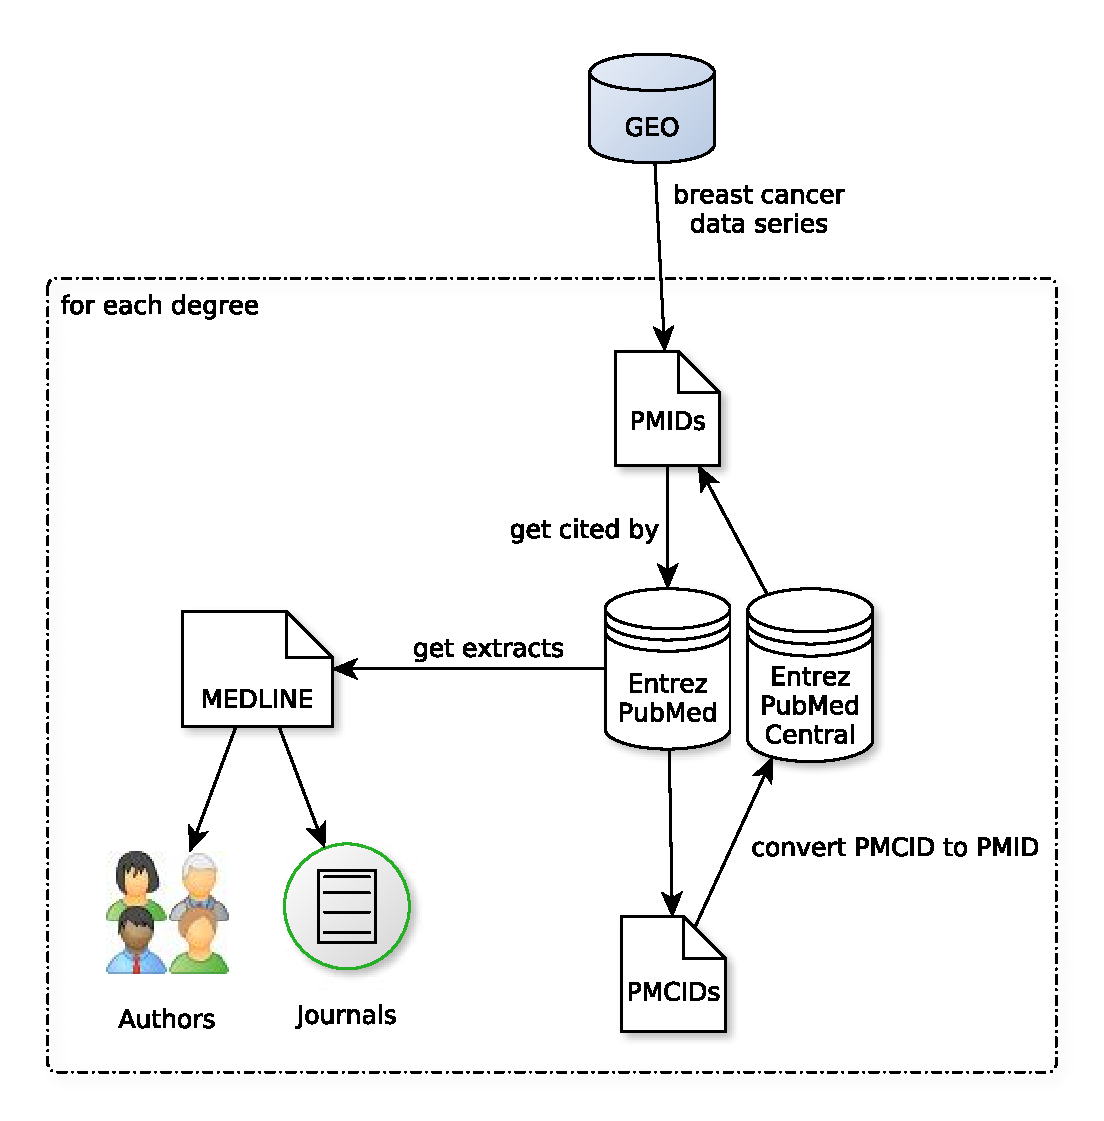
\includegraphics[width=\columnwidth]{ncbi_pipeline.eps}
    \caption{NCBI Query Pipeline}
    \label{fig:pipeline}
\end{figure}

From this, two preprocessing steps occur before arriving at the data used in our experiments. First, we only look at up to the first three authors plus the last author of a paper. Because of the interdisciplinary nature of biomedicine, many publications may consist of more than 20 authors or committees of people within an institution. The last author is used because it oftentimes corresponds to an adviser for the paper. Without a cap on four authors per paper, we expect the number of authors to increase following the paper size increase until the entire community is accounted. From this 57,332 author subset, we then delete 34,638 authors who had less than two papers in our corpus. Both of these choices are done to decrease the sparsity of our transition matrices and to obtain what we consider the important contributors for a paper. Second, we restrict the data to papers and authors attached to the top 100 journals, which include around 40\% of the publications and 50\% of the author subset. We make this restriction on journal number to increase the density of the tensors used in the multirank framework, where we have used journal as the relation connecting authors. After preprocessing, our data consists of 9,451 papers, associated with 9 datasets, written in 100 journals by 11,448 authors.

As a comparison, raw data used for the current DataRank prototype (queried in May 2014) contains around 2.7 million papers with 2,835,252 unique authors and 20,483 journals. From this, only 20,000 datasets are indexed, so the paper and author space is diminished significantly. We believe our experiments on a data size one hundredth of the size of unprocessed data used in DataRank is satisfactory for our exploratory methods to enhance the feature selection and ranking process of the existing prototype.

\paragraph{Data Statistics}
The following information gives a sense of the boundaries of our data to put into context the numbers shown in Result tables found in Section~\ref{sec:results}.

\begin{itemize}[noitemsep,nolistsep]
    \item Highest \# of publications: 28
    \item Authors with highest \# of publications: Perou, Charles M and Creighton, Chad J
    \item Mean number of paper per author: 2.13
    \item Median number of paper per author: 2
    \item Number of authors with no collaborators: 2,627
    \item Average number of collaborators for authors \footnote{authors with collaborations}: 3.58
    \item Highest number of collaborators: 44 for Creighton, Chad J
    \item Mean number of journals in which author is published: 1.83
    \item Mean number of papers per journal \footnote{of the top 100 journals}: 103.44
    \item Median number of papers per journal: 52.5
    \item Max/Min number of papers per journal: 1692 / 8
    \item Highest cited by count for PMID: 519
    \item Mean of cited by count for PMID: 13.04
    \item Median of cited by count for PMID: 5
\end{itemize}

\subsection{Corank}
Corank uses five parameters, but we set three parameters ($m,n,k = 1$) to simplify the implementation to only take into account two parameters: $\alpha = 0.1$ and $\lambda = 0.2$. The implicit parameters correspond to the number of intra-class and inter-class steps taken. With $k=1$, the inter-walk procedure in Algorithm~\ref{alg:inter} takes three substeps ($2k+1$). The authors of Corank suggest preventing large $k$ because it would eliminate the effects between authors and papers. The number of intra-class steps taken is governed by parameters $n,m$ for the citation and author network, respectively. Increasing these parameters means taking powers of $\tilde{A}^T$ and $\tilde{P}^T$ when updating $\mathbf{a}$ and $\mathbf{d}$ in Algorithm~\ref{alg:corank}. Changing these parameters did not greatly affect the top 20 authors or papers in the original corank experiments, so we set them to 1 for faster computation. As explained previously, $\alpha$ is like the dampening parameter used in PageRank that gives the probability a web surfer will continue clicking; the analogous value assumed in PageRank is 0.15. A larger $\alpha$ parameter would cause the transition matrices to be closer to uniform. $\lambda$ is the coupling factor for the random walks; the extremes of $\lambda=0,1$ correspond to taking either only intra-class walks or inter-class walks. 


\subsection{MultiRank}
Unlike Corank, there are no parameters needed --- only the definition of the tensor is required to implement Multirank. We define tensor $\mathcal{A}$ as author citations through journals, where authors act as objects and journals as relations. Thus the value of $a_{i_1,i_2,j_1}$ counts the instances where a paper written by author $i_1$ is cited by a paper written by author $i_2$ and both papers are published in journal $j_1$. Additionally, we restrict these counts to prevent self-citations such that $a_{i1,i1,j1} = 0$ for all authors and journal relations. With this representation, $\mathcal{A}$ is of size 11,448 by 11,448 by 100. Disregarding dangling nodes, $\mathcal{A}$ contains 15,021 non-zero entries, so the sparsity density is $1.146 \times 10^{-6} \%$. Our output is two ranking vectors $\mathbf{x}\in \mathbb{R}^{11448}$ and $\mathbf{y} \in \mathbb{R}^{100}$. The ranking for vector $\mathbf{x'}$ is disregarded because our data is only generated from a `cited by' relationship, rather than a `cites' relationship, though both vectors are used in the iterative algorithm. 

\paragraph{Sparsity Issue}
With such a highly sparse tensor, many of the tensor entries needed to be set as dangling nodes with the probability $\frac{1}{d}$. Filling in these entries resulted in a huge tensor, so an alternative method of computing the probabilities in equations~\ref{eq:vec_x} and~\ref{eq:vec_y} is required to deal with the dangling node issue. This is done by using linear indices, saving the the indices of non-dangling nodes and dangling nodes, and computing each entry of the stationary probability as a non-dangling portion plus the dangling portion. Since the dangling portion is constant, it can be precomputed and reused. 

We show the calculation for $\mathbf{x}$ as an example and make use of MATLAB's conversion of matrix subscripts to linear indices. For a particular $i_1$,

\begin{align*}
    x_i &= \sum_{i_2,j_1} \hat{O}_{i,i_2,j_1} M_{i_2,j_1} \\
                &= \textsc{sub2ind}(\hat{O}_{i,:,:})^T \textsc{sub2ind}(M) \\
                &= \textsc{sub2ind}(O_{i,idx})^T \textsc{sub2ind}(M(idx)) + \frac{1}{m} \sum_{i_2,j} M(dng) 
\end{align*}

where $M=\mathbf{xy^T}$ and $$
\hat{O}_{i,i_2,j_1} =
\begin{cases}
O_{i,i_2,j_1}, & i_2,j \in \text{idx} \\
\frac{1}{m}, & i_2,j \in \text{dng}
\end{cases} $$
